\documentclass{beamer} 
\usepackage{beamerthemesplit} 
\usepackage{wrapfig} 
\usepackage{verbatim} 
\usetheme{SPbGU} 
\usepackage{pdfpages} 
\usepackage{amsmath} 
\usepackage{cmap}
\usepackage{array} 
\usepackage[T2A]{fontenc} 
\usepackage[utf8]{inputenc} 
\usepackage[english,russian]{babel} 
\usepackage{indentfirst} 
\usepackage{amsmath} 
\usepackage{tikz} 
\usepackage{multirow} 
\usepackage[noend]{algpseudocode} 
\usepackage{algorithm} 
\usepackage{algorithmicx} 
\usetikzlibrary{shapes,arrows} 
\usepackage{fancyvrb} 
\usepackage{tikz} 
\usepackage{pgfplots} 
\usepackage{sidecap} 
\usepackage{soul}
\usepackage{xcolor}
\usepackage{tabu}
\usepackage{colortbl}
\pgfplotsset{compat=1.9} 
\newtheorem{rutheorem}{Теорема} 
\newtheorem{ruproof}{Доказательство} 
\newtheorem{rudefinition}{Определение} 
\newtheorem{rulemma}{Лемма} 
\beamertemplatenavigationsymbolsempty 

\newcounter{NoTableEntry}
\renewcommand*{\theNoTableEntry}{NTE-\the\value{NoTableEntry}}

\newcommand*{\strike}[2]{%
	\multicolumn{1}{#1}{%
		\stepcounter{NoTableEntry}%
		\vadjust pre{\zsavepos{\theNoTableEntry t}}% top
		\vadjust{\zsavepos{\theNoTableEntry b}}% bottom
		\zsavepos{\theNoTableEntry l}% left
		\hspace{0pt plus 1filll}%
		#2% content
		\hspace{0pt plus 1filll}%
		\zsavepos{\theNoTableEntry r}% right
		\tikz[overlay]{%
			\draw
			let
			\n{llx}={\zposx{\theNoTableEntry l}sp-\zposx{\theNoTableEntry r}sp-\tabcolsep},
			\n{urx}={\tabcolsep},
			\n{lly}={\zposy{\theNoTableEntry b}sp-\zposy{\theNoTableEntry r}sp},
			\n{ury}={\zposy{\theNoTableEntry t}sp-\zposy{\theNoTableEntry r}sp}
			in
			(\n{llx}, \n{lly}) -- (\n{urx}, \n{ury})
			;
		}% 
	}%
}

\title[]{Extended Context-Free Grammars Parsing with Generalized LL} 
% То, что в квадратных скобках, отображается в левом нижнем углу. 
\institute[SPBU]{ 
	Saint Petersburg State University \\ 
	Programming Languages and Tools Lab, JetBrains} 

% То, что в квадратных скобках, отображается в левом нижнем углу. 
\author[Artem Gorokhov]{Artem Gorokhov} 
\date{March 4 2017} 

\begin{document} 
	
	\definecolor{red}{RGB}{255,0,0} 
	
	\begin{frame} 
		\begin{center} 
			{
\includegraphics[width=1.5cm]{pictures/SPbGU_Logo.png}} 
		\end{center} 
		\titlepage 
		%Hello, My name is Artem
		%Im from Jetbrains programming languages and tools laboratory
		%I would like to tell you about 
		%Extended Context-Free Grammars Parsing with Generalized LL Algorithm
	\end{frame}

	\begin{frame}
		\begin{center} 
			{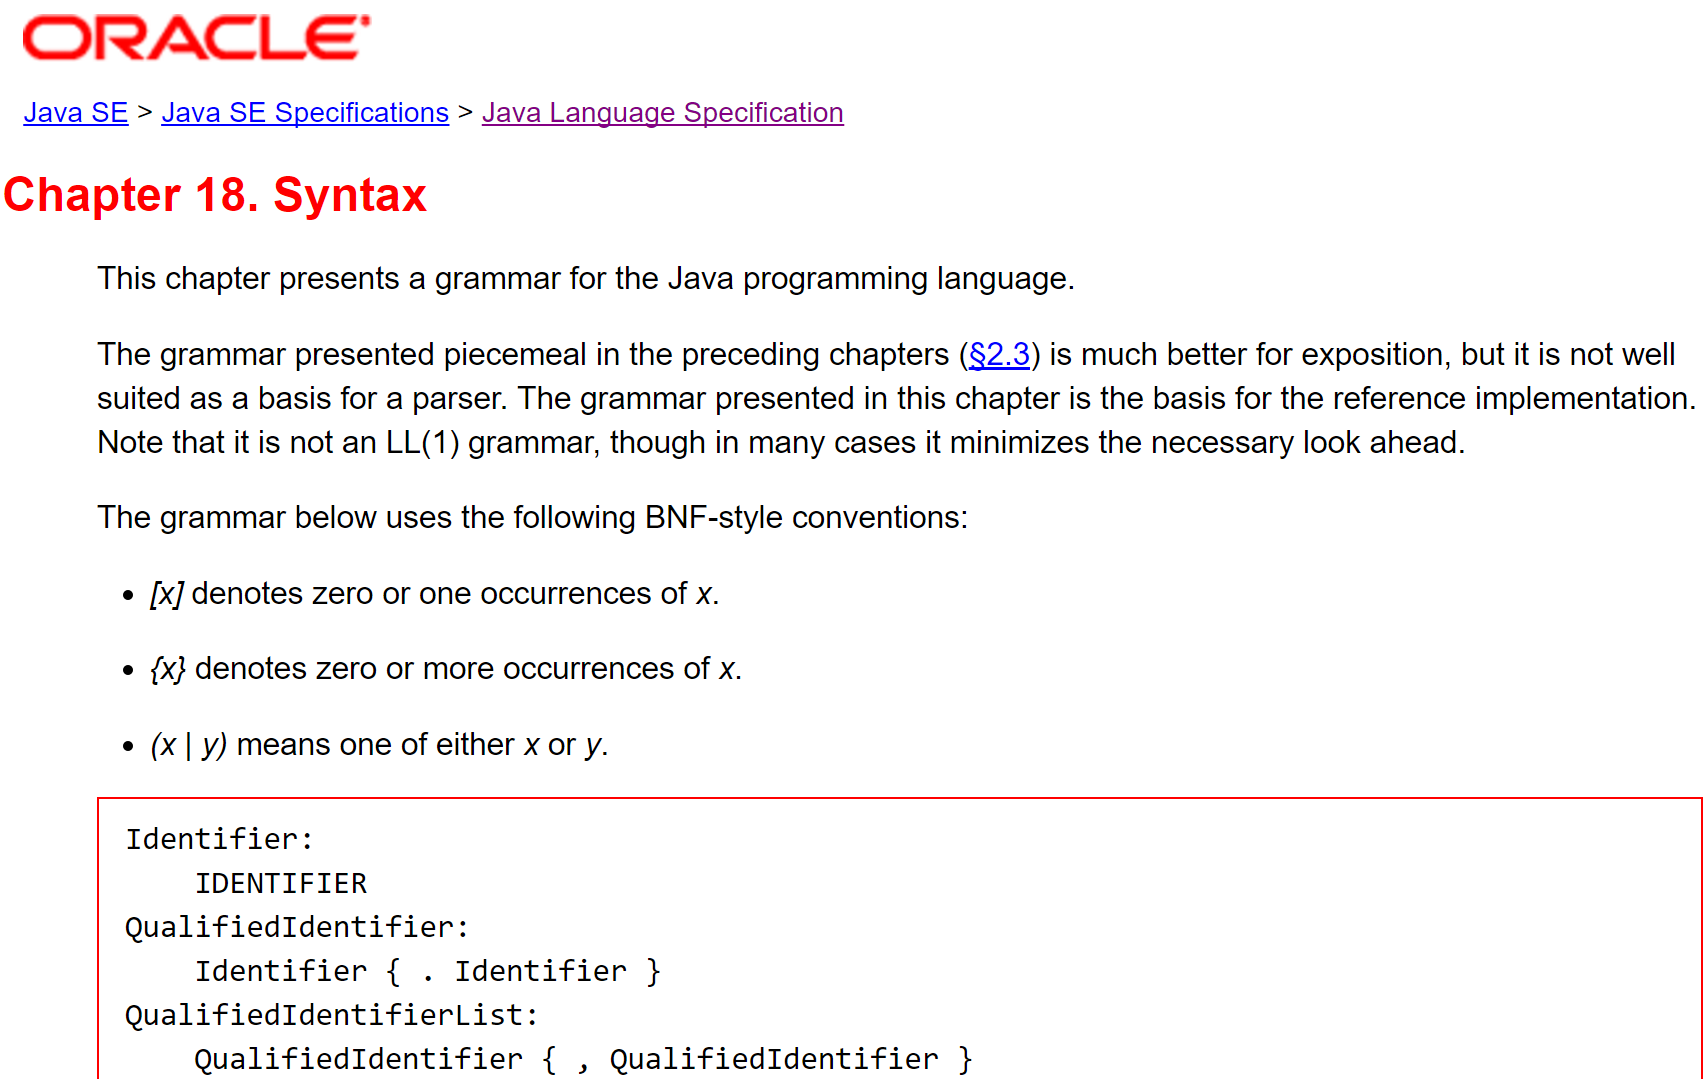
\includegraphics[width=12cm]{pictures/java_grammar.png}} 
		\end{center}
		\iffalse
		In documentation most common way to express grammars is different variations of EBNF notation.
		And it is naturally because it is more human-readable than BNF. 
		
		
		The problem is that original GLL algorithm admits only BNF grammars: 
		there should be only alternations of sequences that consists of terminals and nonterminals. 
		when a most common way to express grammars in documentation is ECFG. In such form
		right-hand sides of grammar productions are regular expressions under alphabet of terminals and nonterminals. 
		It is more widely known as EBNF. It is the same form in
		respect to construction names. consequence of this problem is grammar transformation 
		transformation leads to grammar size increase and change in grammar
		structure: new nonterminals are added during transformation. As a result, parser
		constructs derivation tree with respect to the transformed grammar, making it
		harder for a language developer to debug grammar and use parsing result later.
		\fi
	\end{frame}

	\begin{frame} 
		\frametitle{Extended Context-Free Grammar}
		\begin{center}
			{$\begin{aligned}
				S\ =&\ a\ M^* \\
				M\ =&\ a?\ (B\ K)^+ \\
				|&\ u\ B \\
				B\ =&\ c\ |\ \varepsilon
				\end{aligned}$}
		\end{center}
		
		
		\iffalse
		EBNF have many notations in real world so to clarify 
		the notation that we will use Extended context free
		grammars. Extended context free grammar is context-free
		grammar whose right-hand sides of productions are 
		regular expressions over alphabet of terminals and nonterminals.
		
		\fi
	\end{frame}
	
	\begin{frame}
		\begin{columns}
			\begin{column}{6.1cm}
				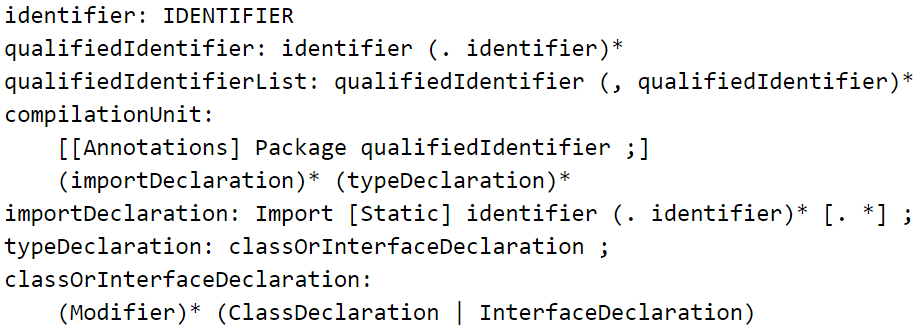
\includegraphics[width=6cm]{pictures/java_before.png}
			\end{column}
			\begin{column}{.7cm}
				$ \Longrightarrow $
			\end{column}
			\begin{column}{5cm}
				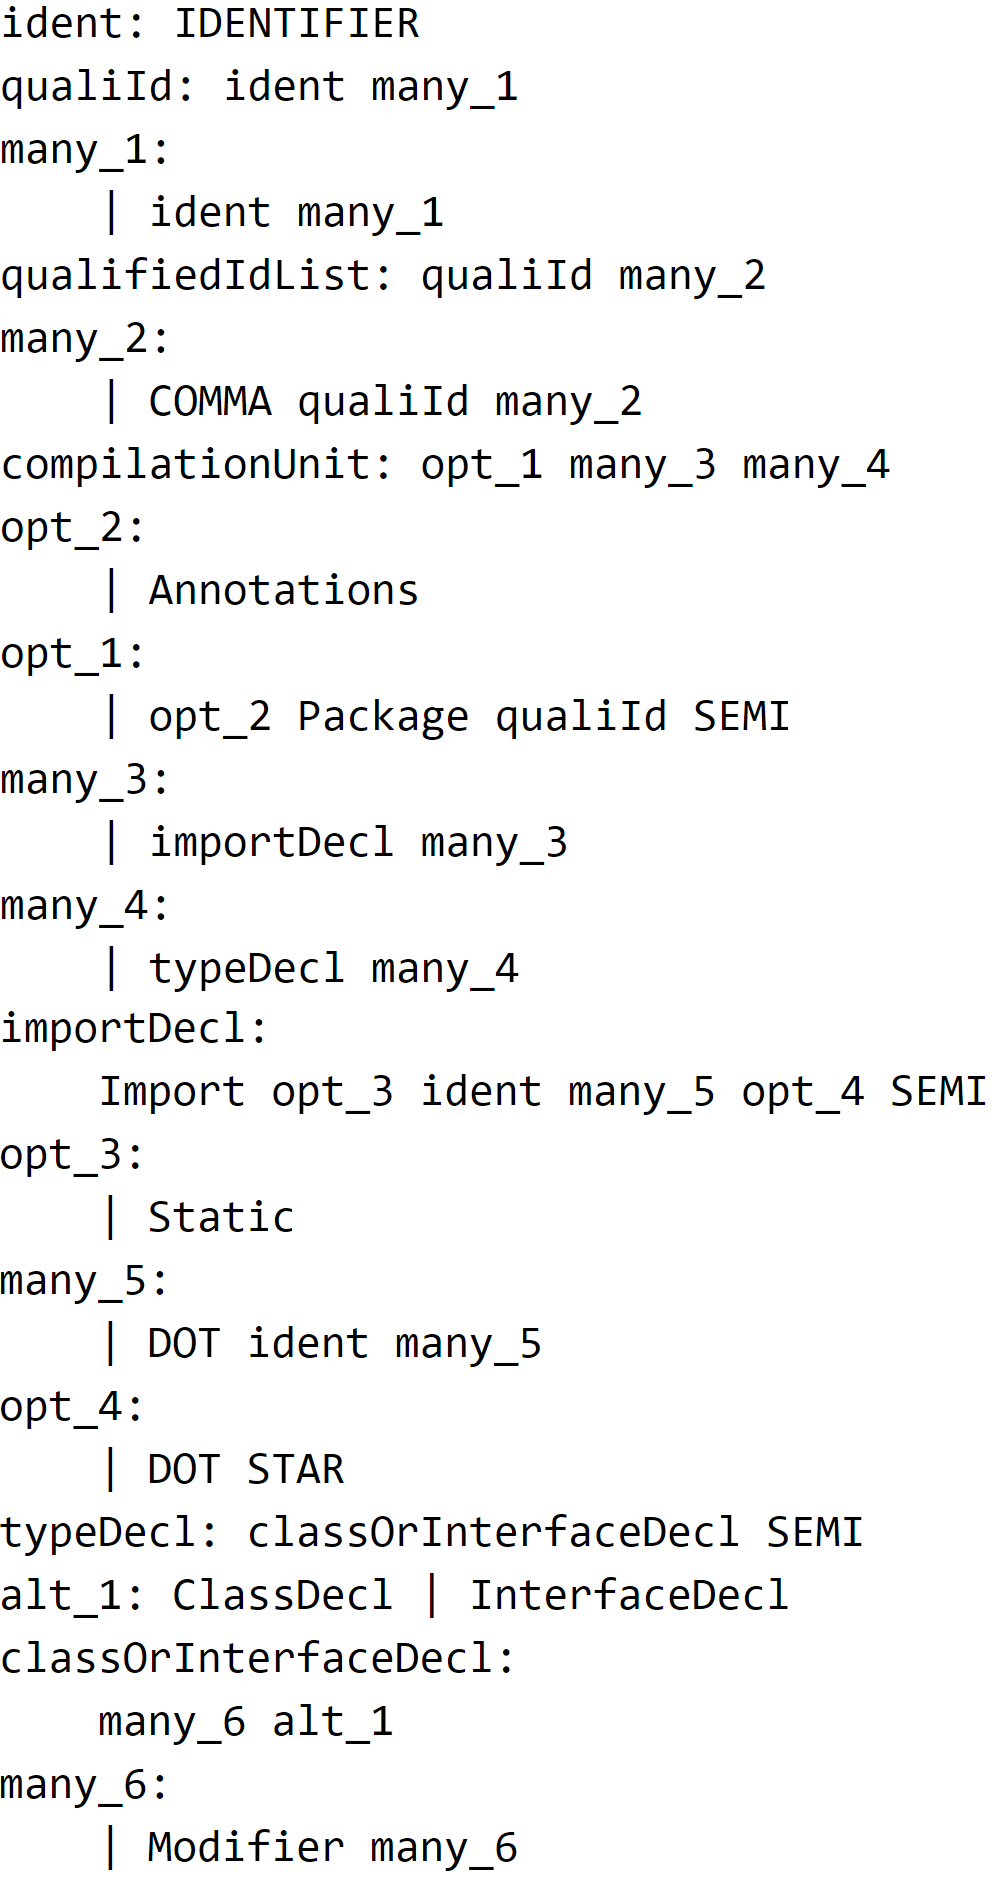
\includegraphics[width=4.8cm]{pictures/java_after.png}
			\end{column}
	    \end{columns}
		\iffalse
		If we transform the grammar in BNF it's size will increase and will get completely lost in it.
		
		But parsers, like people, are sensitive to grammar size.
		With grammar size increase, the time of parsing increases as well. 
		But most of the algorithms are use grammars in BNF.
		So to use them we need to convert grammar to BNF.
		Other consequence of such transformation is change in
		grammar structure, and parser constructs derivation tree
		with respect to the transformed grammar, making it
		harder for a language developer to debug grammar and use
		parsing result later.
		\fi
	\end{frame}

\begin{frame}
	\begin{center} 
		\only<1>{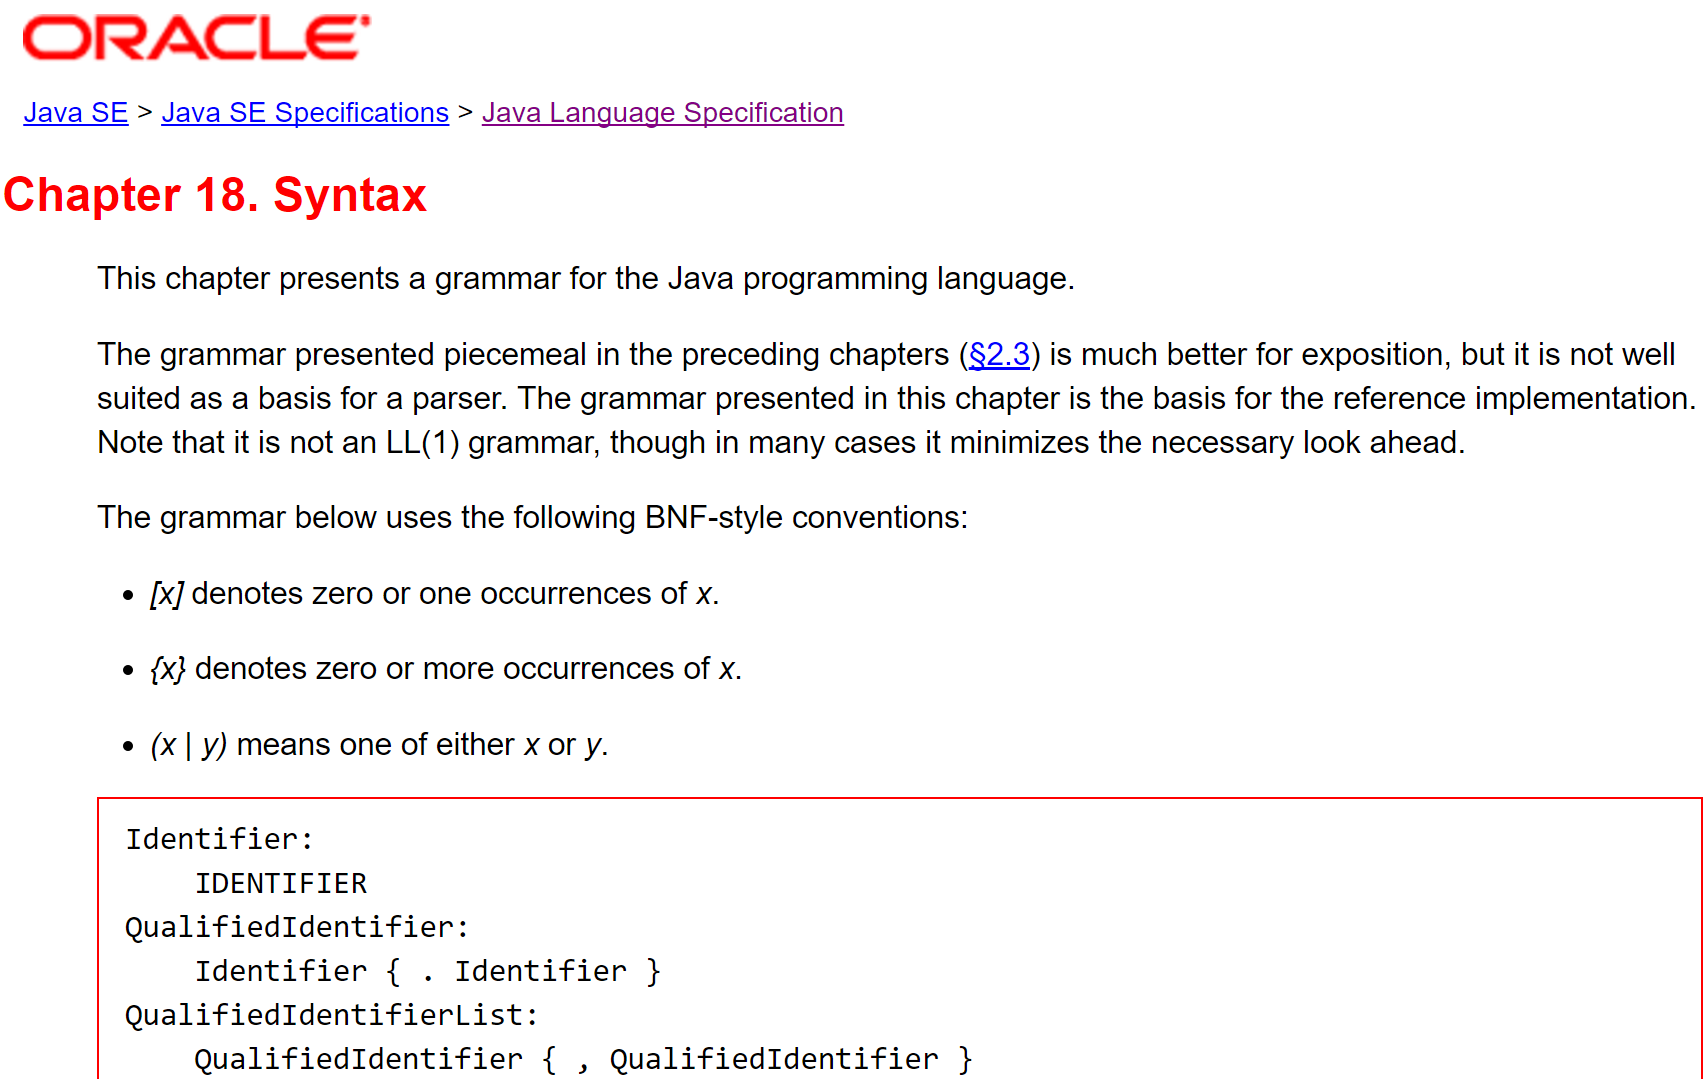
\includegraphics[width=12cm]{pictures/java_grammar.png}} 
		\only<2>{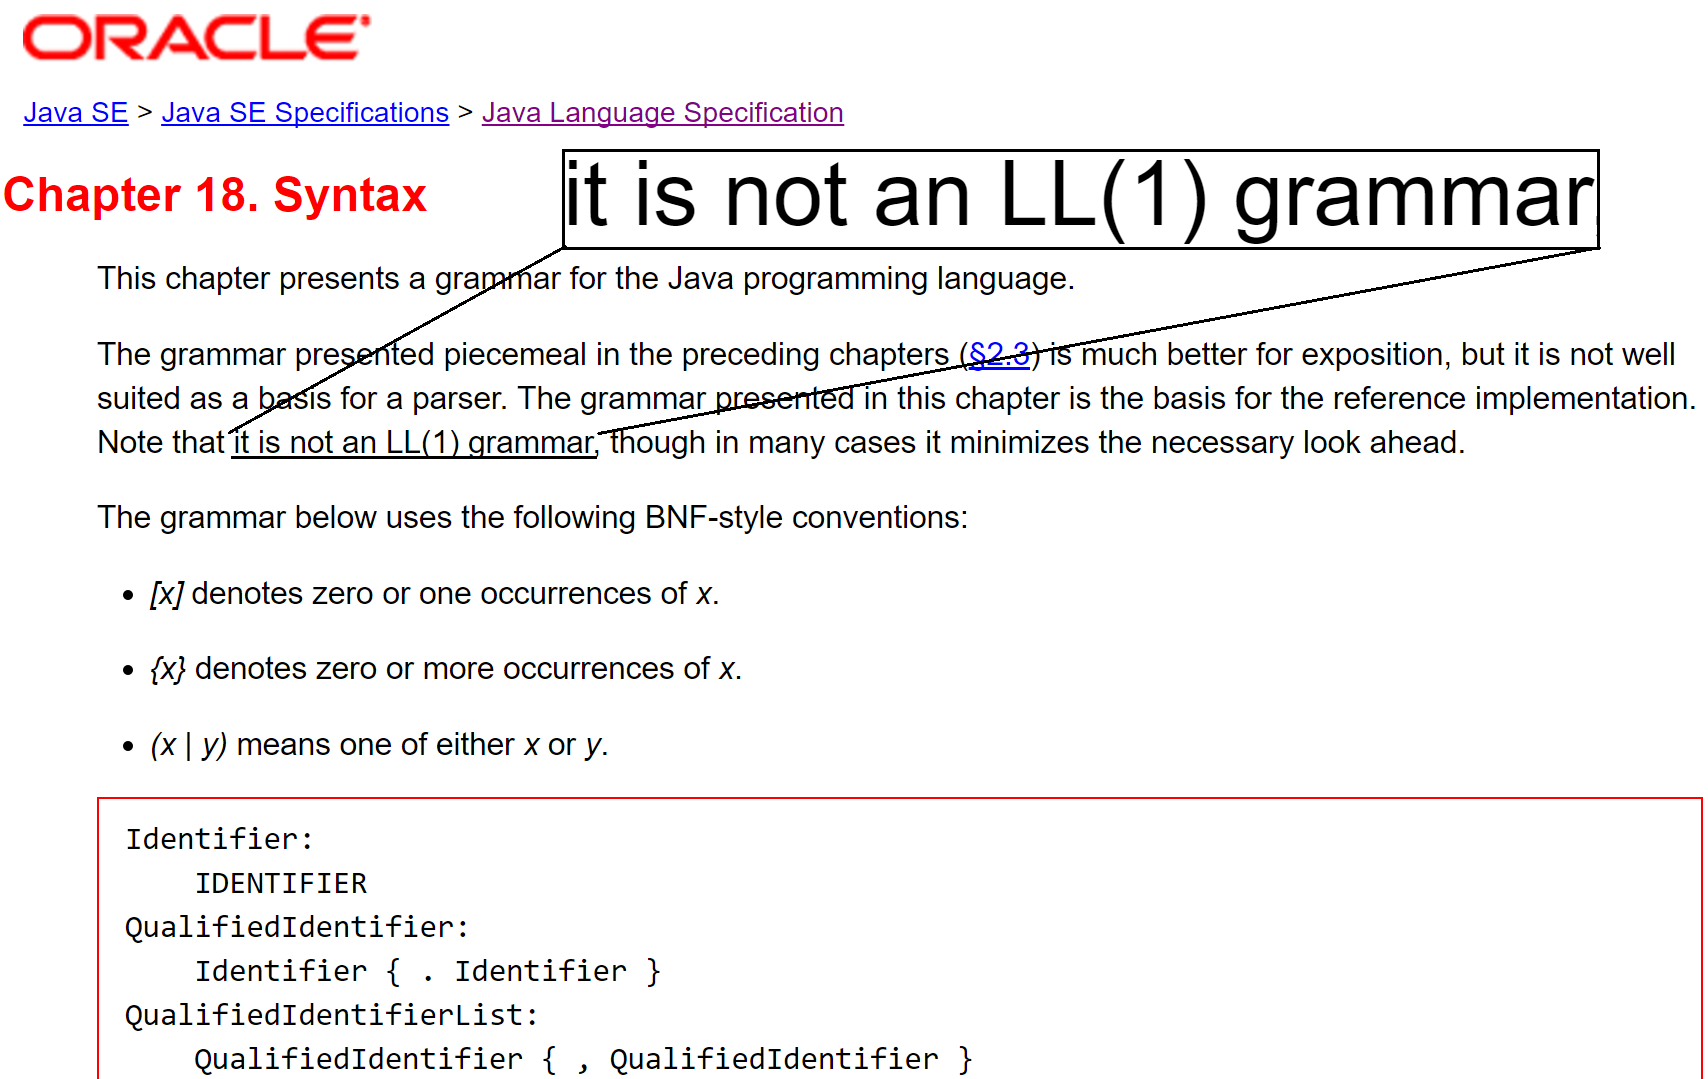
\includegraphics[width=12cm]{pictures/java_grammar_2.png}} 
	\end{center}
	\iffalse
	In documentation most common way to express grammars is different variations of EBNF notation.
	And it is naturally because it is more human-readable than BNF. 
	
	
	The problem is that original GLL algorithm admits only BNF grammars: 
	there should be only alternations of sequences that consists of terminals and nonterminals. 
	when a most common way to express grammars in documentation is ECFG. In such form
	right-hand sides of grammar productions are regular expressions under alphabet of terminals and nonterminals. 
	It is more widely known as EBNF. It is the same form in
	respect to construction names. consequence of this problem is grammar transformation 
	transformation leads to grammar size increase and change in grammar
	structure: new nonterminals are added during transformation. As a result, parser
	constructs derivation tree with respect to the transformed grammar, making it
	harder for a language developer to debug grammar and use parsing result later.
	\fi
\end{frame}

	

	\begin{frame} 
		\frametitle{Existing solutions} 
		\begin{itemize}
			\item<1-> ANTLR, Yacc, Bison
			 \begin{itemize}
			 	\item<2-> Can't use ECFG without transformation
			 	\item<2-> Admit only subclass of ECFG (LL(k), LR(k))
			 \end{itemize} 
			\item<3-> Some research on ECFG parsing
			\begin{itemize}
				\item<4-> No tools
				\item<4-> LL(k), LR(k)
			\end{itemize}
			\item<5-> \only<5-6>{Generalized LL}\only<7>{\textbf{Generalized LL}}
			\begin{itemize}
				\item<6-> Admit arbitrary CFG(including ambiguous)
				\item<6-> Can't use ECFG without transformation
			\end{itemize}
		\end{itemize}
		\iffalse
		On the other hand there is a wide range of parsing
		techniques and algorithms that are able to process ECF grammars. 
		But most of them are based on classical LL and LR techniques,
		so they admit only restricted subclasses of ECFG. Thus, there
		is no solution for handling arbitrary ECFG. 
		
		GLL is top-down parsing algorithm that
		parses the input from Left to right, 
		building Leftmost derivation of the input.
		But unlike the LL algorithm that admit only
		subset of context free grammars GLL
		allows arbitrary context free grammars
		thus, in case of ambiguity in grammar, 
		parser builds parse forest that represent
		all possible derivations of input
		
		but the problem is that it works only with BNF grammars
		\fi
	\end{frame}

	\begin{frame} 
		\frametitle{Automata and ECFGs}
		
		\begin{columns}
			\begin{column}{4cm}
				Grammar $G_0$\\
				\vspace{10pt}
				$
				\begin{array}[b]{rl}
				S = a^{*} S\ b? \ | \ c \ \ \ \ \ \ \ \ \  \Longrightarrow
				\end{array}
				$
			\end{column}
			\begin{column}{3cm}
				RA for grammar $G_0$\\
				\vspace{10pt}
				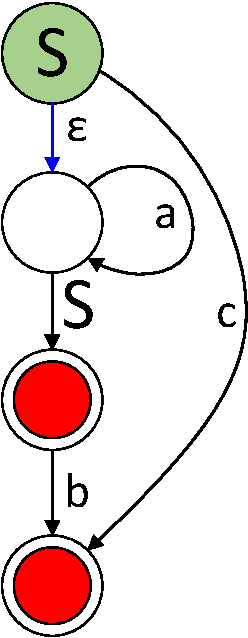
\includegraphics[width=2.5cm]{pictures/G0initialAutomaton.pdf}
			\end{column}
		\end{columns}
		\iffalse
		As I mentioned before, ECF grammar's right-hand
		sides of productions are regular expressions.
		So we can easily convert them to automata
		
		Such (WHAT) is called Recursive Automata.
		So it is just FSA whose transitions can be 
		not only by terminals, but also by nonterminals 
		\fi
	\end{frame}

	\begin{frame} 
		\frametitle{Recursive Automata Minimization}
		\vspace{-12pt}
		\begin{center}
			%\begin{tabular}{c}
			{Grammar $G_1$\\
			\vspace{5pt}
			$
			\begin{array}{rl}
			S =& K\ K\ K\ K\ K\ K \ |K\ a\ K\ K\ K\ K \\
			K =& S\ K\ |\ a\ K\ |\ a \\
			\end{array}
			$
			}
		    \\
		    \vspace{12pt}
		    Automaton for $G_1$
		    \\
		    \vspace{5pt}
		    {
				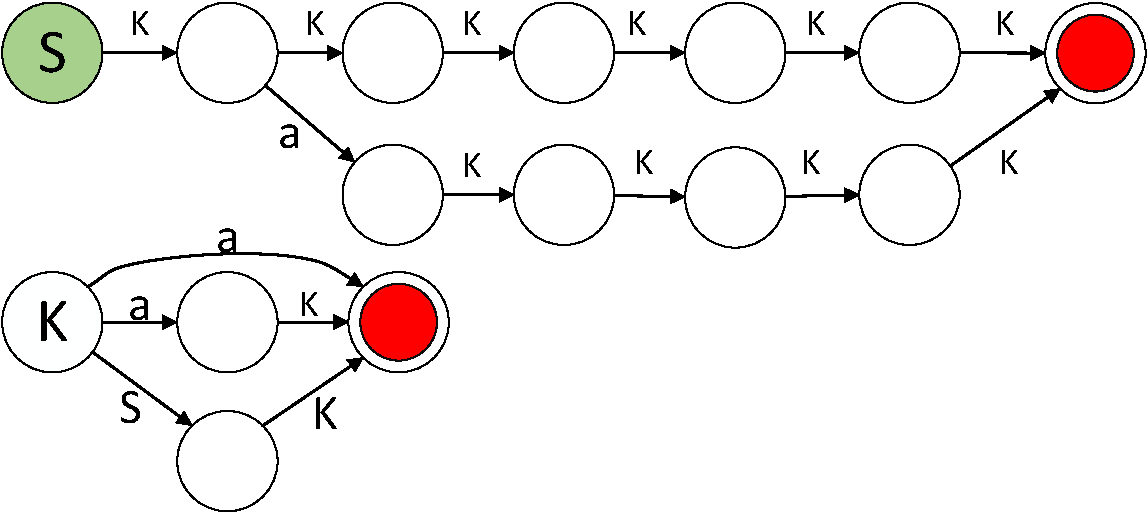
\includegraphics[width=7cm]{pictures/G1initial.pdf}
			}\\
			\vspace{8pt}
			Minimized automaton for $G_1$
			\\
			\vspace{5pt}
		    {
				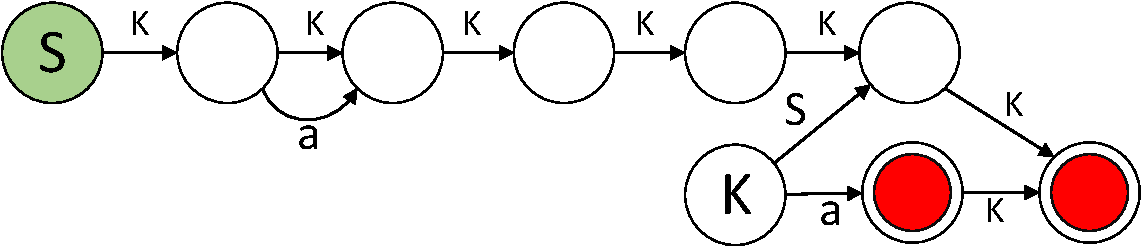
\includegraphics[width=7cm]{pictures/G1automaton.pdf}
			}
		\end{center}
		\iffalse
		Why RA? Because in fact, we can apply any well known FSA minimization algorithms to RA.
		%But with minimithation the structure will be the same because we just merge equivalent states
		So we can get minimized (by state number) deterministic RA.
		And this minimization can significantly increase parsing performance 
		\fi
	\end{frame}
	
	\begin{frame} 
		\frametitle{Derivation Trees for Recursive Automata}
		%\vspace{-40pt}
		\begin{columns}
			\begin{column}{3.7cm}
				%Grammar: $$ S : a^{+} S\ b? \ | \ c $$
				Input: $$aacb$$ \\
				\vspace{10pt}
				Automaton: \\
				\vspace{5pt}
				\begin{center}
					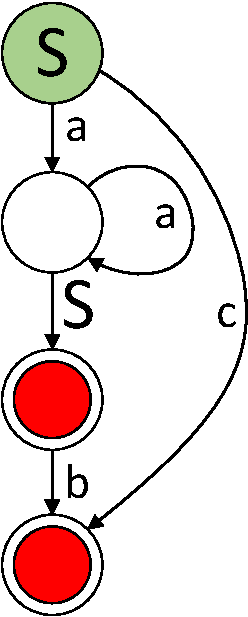
\includegraphics[width=2cm]{pictures/G0minimizedAutomaton.pdf}
				\end{center}
			\end{column}
		
     		\begin{column}{6cm}
     			\ \ Derivation trees:\\
     			\vspace{5pt}
     			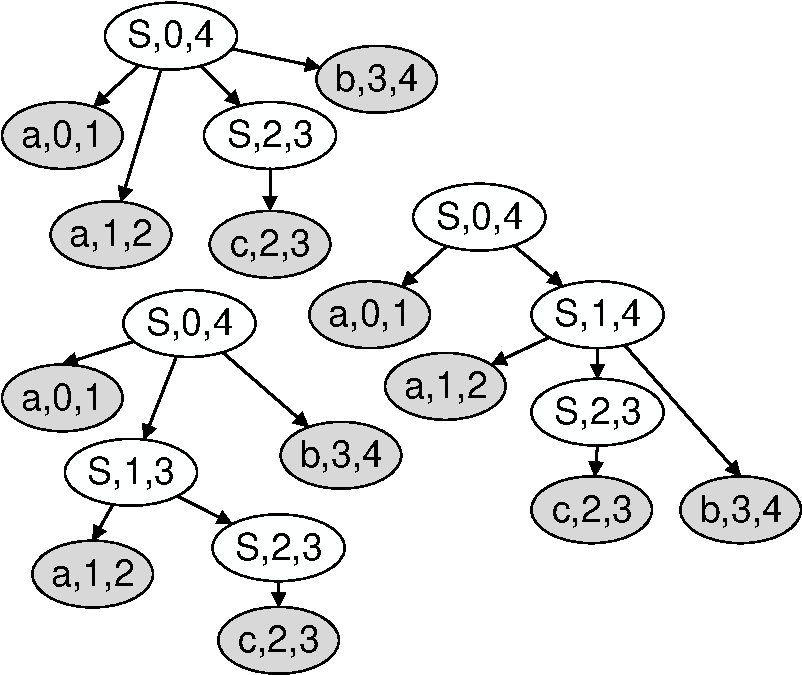
\includegraphics[width=7cm]{pictures/G0trees.pdf}
			\end{column}
		
		\end{columns}
		\iffalse
		Now we have convenient representation of our grammar as RA
		But we need to define Parse forest for it
		Firstly we can define tree for RA
		It is ordered rooted tree which root is labeled with start state
		leaves are terminals
		Nodes are nonterminals
		And nonterminals have sequence of children if there exists path
		which starts in first state of this nonterminal
		\fi
	\end{frame}
	
	\begin{frame} 
		\frametitle{SPPF for Recursive Automata}
		\begin{columns}
			\begin{column}{5cm}
				%Grammar: $$ S : a^{+} S\ b? \ | \ c $$
				Input: $$aacb$$ \\
				\vspace{10pt}
				Automaton: \\
				\vspace{5pt}
				\begin{center}
					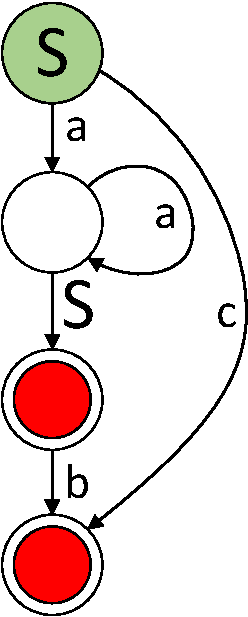
\includegraphics[width=2cm]{pictures/G0minimizedAutomaton.pdf}
				\end{center}
			\end{column}
			\begin{column}{6cm}
				Shared Packed Parse Forest: \\
				\vspace{10pt}
				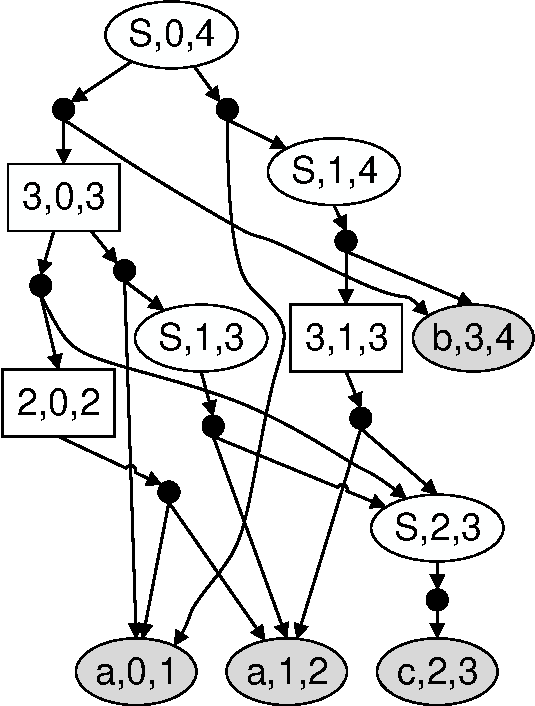
\includegraphics[width=5cm]{pictures/G0SPPF.pdf}
				\\
				Mb highlight each tree?
			\end{column}
		\end{columns}
		\iffalse
		
		\fi
	\end{frame}
	
	\begin{frame} 
		\frametitle{Input processing}
		\begin{itemize}
			\item Descriptors queue
			\item Descriptor (G, i, U, T) uniquely defines parsing process state
			\begin{itemize}
				\item G - \only<1>{position in grammar}
						  \only<2>{\st{position in grammar}\ \  state of RA}
				\item i - position in input
				\item U - stack node
				\item T - current parse forest root
			\end{itemize}
		\iffalse
		So, now we have grammar representation and we know what we should construct
		Firstly, because we changed grammar to RA we need to 
		represent new descriptor
		The tuple (S, U, i, N) where S is state of A. other elements doesn't change 
		\fi
		\end{itemize}
		
	\end{frame}
	\begin{frame} 
		\frametitle{Input processing}
		\begin{columns}
			\begin{column}{5cm}
				Input : $\only<1-2>{\ \ }\only<3->{\bullet} \ b c $ \\
				\vspace{15pt}
				Grammar: \\
				\vspace{5pt}
				\only<1>{$$
					S = \ (a\ |\ b\ |\ S)\ c?
					$$}
				\only<2->{$
				\begin{array}{rl}
				S =&\only<3>{\bullet} \ a\ C\_opt \\
				|&\only<4>{\bullet} \ b\ C\_opt \\
				|&\only<5>{\bullet} \ S\ C\_opt \\
				C\_opt =& \varepsilon \ | \ c \\
				\end{array}
				$}
			\end{column}
			\begin{column}{5cm}
				\only<3->{
				\begin{tabu}{|[3pt]c|[3pt]}
					\only<5->{$S =\bullet \ S\ C\_opt$, 0, \dots, \dots \\
					\hline}
					\only<3-4>{$\ \ \ \ \ \ \ \ \ \ \ \ \ \ \ \ \ \ \ \ \ \ \ \ \ \ \ \ \ \ \ \ \ \ $ \\}
					%\strike{|[3pt]c|}{quux} & A & B \\
					\only<4->{$S =\bullet \ b\ C\_opt$, 0, \dots, \dots \\
					\hline}
					\only<3>{$\ \ \ \ \ \ \ \ \ \ \ \ \ \ \ \ \ \ \ \ \ \ \ \ \ \ \ \ \ \ \ \ \ \ $ \\}
					\only<3-5>{$S =\bullet \ a\ C\_opt$, 0, \dots, \dots}
					\only<6>{\cellcolor{blue!25}{ $S =\bullet \ a\ C\_opt$, 0, \dots, \dots}}
				\end{tabu}
			}
			\end{column}
		\end{columns}
		\iffalse
		for such example in initial algorithm state we will have
		queue consists of 3 descriptors that defines start of input and 
		start of each of 3 productions
		
		Thus the main changes in algorithm are because of changing grammar to RA
		It brings such consequences:
		for a position in grammar we have the only way to move. But for the automaton we can have multiple transitions
		More over current state can be a final state.  
		
		
		for the grammar case it is simple
		we just move in production if it matches the input, creating 
		intermediate sppf nodes and when we reach end of production we 
		construct nonterminal node
		but for the automaton case things become more complicated
		we can have different transitions from current state
		we should handle nonterminal transition and terminal that matches the input token.
		more over if the next state is final we should construct nonterminal node in addition to intermediate and continue derivation for both cases. 
		\fi
	\end{frame}
	\begin{frame} 
		\frametitle{Input processing}
		\begin{columns}
			\begin{column}{5cm}
				Input : $\only<1>{\ \ }\only<2->{\bullet} \ b c $ \\
				\vspace{15pt}
				Automaton : \\
				\vspace{5pt}
				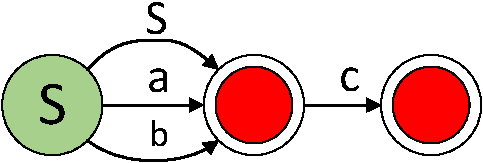
\includegraphics[width=5cm]{pictures/G2.pdf}
			\end{column}
			\begin{column}{5cm}
				\begin{tabu}{|[3pt]c|[3pt]}
					$S =\bullet \ S\ C\_opt$, 0, \dots, \dots \\
					\hline
					%\strike{|[3pt]c|}{quux} & A & B \\
					
					$S =\bullet \ b\ C\_opt$, 0, \dots, \dots \\
					\hline
					$S =\bullet \ a\ C\_opt$, 0, \dots, \dots
				\end{tabu}
			\end{column}
		\end{columns}
		\iffalse
		for such example in initial algorithm state we will have
		queue consists of 3 descriptors that defines start of input and 
		start of each of 3 productions
		
		Thus the main changes in algorithm are because of changing grammar to RA
		It brings such consequences:
		for a position in grammar we have the only way to move. But for the automaton we can have multiple transitions
		More over current state can be a final state.  
		
		
		for the grammar case it is simple
		we just move in production if it matches the input, creating 
		intermediate sppf nodes and when we reach end of production we 
		construct nonterminal node
		but for the automaton case things become more complicated
		we can have different transitions from current state
		we should handle nonterminal transition and terminal that matches the input token.
		more over if the next state is final we should construct nonterminal node in addition to intermediate and continue derivation for both cases. 
		\fi
	\end{frame}
	
	\begin{frame} 
		\frametitle{Evaluation}
		\begin{center}
		\vspace{-10pt}
		Grammar $G_1$\\
		\vspace{6pt}
		$
		\begin{array}{rl}
		S =& K\ K\ K\ K\ K\ K \ | K\ a\ K\ K\ K\ K \\
		K =& S\ K\ |\ a\ K\ |\ a \\
		\end{array}
		$
		\\
		\vspace{15pt}
		RA for grammar $G_1$
		\\
		\vspace{6pt}
		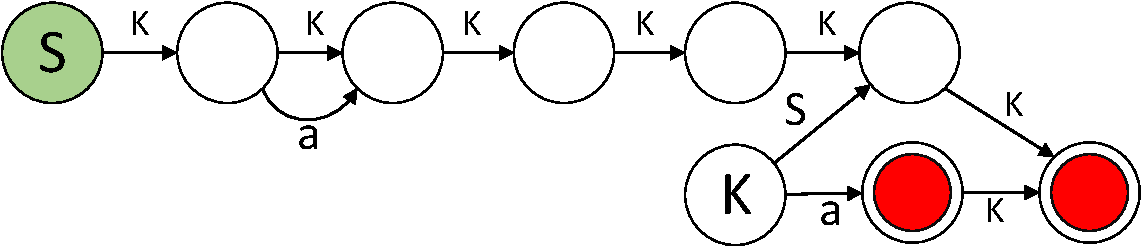
\includegraphics[scale=.5]{pictures/G1automaton.pdf}
		\\
		\vspace{7pt}
		Experiment results for input $a^{40}$
		\\
		\vspace{2pt}
		\begin{tabular}{ | c | c | c | c | c | }
			\hline
             &  Descriptors & Stack Edges & Stack Nodes & SPPF Nodes   \\ \hline
			BNF Grammar  &  7,940        & 6,974      & 80        & 111,127,244  \\ \hline
			Minimized RA &  5,830        & 4,234      & 80        & 74,292,078  \\ \hline \hline
			Difference   &  27$\%$       & 39$\%$     & 0 $\%$    &  33 $\%$ \\ \hline
		\end{tabular}
		\end{center}
	\end{frame}
	
	\begin{frame} 
		\frametitle{Why did we make it?} 
		\begin{center}
		Graph parsing results
		\begin{tabular}{ | c | c | c | c | c | }
			\hline
			             &  Descriptors & Stack Edges & Stack Nodes & Time, min   \\ \hline
			BNF Grammar  &  21,134,080       & 7,482,789      & 2,731,529      & 02.26  \\ \hline
			Minimized RA &  9,153,352        &  2,792,330     & 839,148        & 01.25  \\ \hline \hline
			Difference   &  57$\%$       & 63$\%$     & 69 $\%$    &  45 $\%$ \\ \hline
		\end{tabular}
		\end{center}
		\iffalse
		In real life parsing in, for example, IDEs takes not so much time that our algorithm will show significant performance increase. 
		But in other areas it might be useful. 
		For example graph parsing. (table with results for m g a) 
		\fi
	\end{frame} 
	
\end{document}